\documentclass[urlcolor=blue,dvipsnames]{beamer}

\usepackage[utf8]{inputenc}
\usepackage{fancybox,fancyvrb}
\usepackage{environ,xspace,empheq}

\usepackage{tikz}
\usetikzlibrary{arrows.meta,decorations.markings,decorations.pathreplacing,fadings,positioning}

\hypersetup{colorlinks,linkcolor=,urlcolor=cyan}

\beamertemplatenavigationsymbolsempty
\setbeamertemplate{footline}[frame number]
\usetheme{Pittsburgh}

\newcommand\enumnum[1]{{\renewcommand{\insertenumlabel}{#1}%
      \usebeamertemplate{enumerate item} \,}}

\newcommand{\grad}{\nabla}
\newcommand{\ih}{\boldsymbol{\hat{\textbf{\i}}}}
\newcommand{\jh}{\boldsymbol{\hat{\textbf{\j}}}}
\newcommand{\vF}{\boldsymbol{\vec{\textbf{F}}}}
\newcommand{\Matlab}{\textsc{Matlab}\xspace}
\newcommand{\Octave}{\textsc{Octave}\xspace}


\title{7.2 \emph{inverse} Laplace Transforms, \\ and application to DEs}

\subtitle{a lesson for MATH F302 Differential Equations}

\author{Ed Bueler, Dept.~of Mathematics and Statistics, UAF}

\date{\tiny \today}


\begin{document}
\setbeamertemplate{itemize item}{$\bullet$}
\setbeamertemplate{itemize subitem}{$\circ$}
\renewcommand{\thefootnote}{{\color{green} \arabic{footnote}}}

\begin{frame}
\titlepage

\centerline{\tiny for textbook: \, D. Zill, \emph{A First Course in Differential Equations with Modeling Applications}, 11th ed.}
%\color{green!40!blue}
\end{frame}

\newcommand{\LL}[1]{\mathcal{L}\left\{#1\right\}}
\newcommand{\LLi}[1]{\mathcal{L}^{-1}\left\{#1\right\}}

\begin{frame}{recall the definition}

\begin{itemize}
\item the \emph{Laplace transform} of a function $f(t)$ defined on $(0,\infty)$ is
    $$\LL{f(t)} = \int_0^\infty e^{-st} f(t)\,dt$$
    \begin{itemize}
    \item this is well defined for $s>c$ if $f(t)$ has exponential order $c$:  $|f(t)| \le M e^{ct}$
    \end{itemize}

\bigskip
\item the result of applying the Laplace transform is a function of s:
    $$\LL{f(t)} = \LL{f}(s) = F(s) \hspace{15mm} \longleftarrow \text{all mean the same}$$
\end{itemize}
\end{frame}


\begin{frame}{the Laplace transform strategy}

\begin{center}
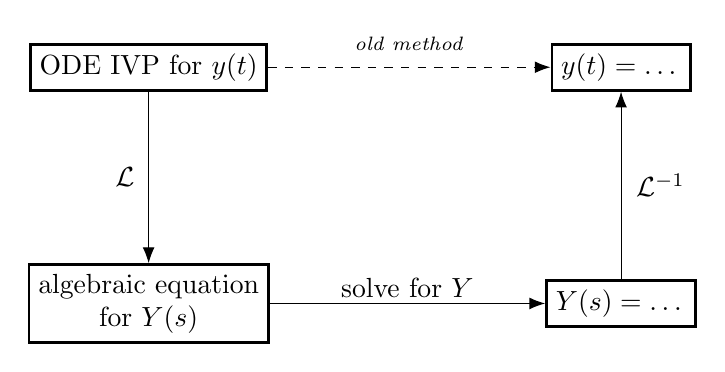
\begin{tikzpicture}[scale=1.0,>={Latex[length=2mm]},
  component/.style={rectangle,draw,fill=white,align=center,line width=1pt}]

\draw (-3,3) node[component] (ode) {ODE IVP for $y(t)$};
\draw (-3,0) node[component] (Leqn) {algebraic equation \\ for $Y(s)$};
\draw (3,0) node[component] (Lsoln)   {$Y(s)=\dots$};
\draw (3,3) node[component] (odesoln)   {$y(t)=\dots$};
\path
   (ode) edge[->] node[xshift=-3mm] {$\mathcal{L}$} (Leqn)
   (Leqn) edge[->] node[yshift=2mm] {solve for $Y$} (Lsoln)
   (Lsoln) edge[->] node[xshift=+5mm] {$\mathcal{L}^{-1}$} (odesoln)
   (ode) edge[dashed,->] node[yshift=3mm] {\scriptsize \emph{old method}} (odesoln);

\end{tikzpicture}
\end{center}

\vspace{10mm}
\begin{itemize}
\item \S 7.2: practice with $\mathcal{L}^{-1}$ then practice the whole strategy
\end{itemize}
\end{frame}


\begin{frame}{bring a table to the party}

\begin{center}
\includegraphics[width=0.75\textwidth]{figs/laplacetable.pdf}
\end{center}

\begin{itemize}
\item on page 282 of book
\item this table is pathetic!  better one soon \dots
\end{itemize}
\end{frame}


\begin{frame}{first $\mathcal{L}^{-1}$ example (like \S7.2 \#5)}

\begin{itemize}
\item \emph{exercise 1.}  use algebra and a table of Laplace transforms:
    $$\LLi{\frac{(s-1)^3}{s^4}} = \hspace{80mm}$$
\end{itemize}

\vspace{50mm}
\end{frame}


\begin{frame}{$\mathcal{L}^{-1}$ example like \S7.2 \#11}

\begin{itemize}
\item \emph{exercise 2.}  use algebra and a table of Laplace transforms:
    $$\LLi{\frac{5}{s^2+36}} = \hspace{80mm}$$
\end{itemize}

\vspace{50mm}
\end{frame}


\begin{frame}{$\mathcal{L}^{-1}$ example like \S7.2 \#18}

\begin{itemize}
\item \emph{exercise 3.}  use algebra and a table of Laplace transforms:
    $$\LLi{\frac{s+1}{s^2-7s}} = \hspace{80mm}$$
\end{itemize}

\vspace{50mm}
\end{frame}


\begin{frame}{not actually a better table}

\begin{itemize}
\item compare Theorems 7.1.1 and 7.2.1
\item they say the same thing!
\end{itemize}

\mbox{\includegraphics[height=40mm]{figs/laplacetable.pdf} \qquad \includegraphics[height=42mm]{figs/inverselaplacetable.pdf}}

\end{frame}


\begin{frame}{actually a better table}

\small
\begin{itemize}
\item this \emph{substantial} table will be printed on your quiz/exam
\end{itemize}

\vspace{-3mm}
\tiny
\begin{minipage}[t]{0.3\textwidth}
\begin{align*}
\LL{1} &= \frac{1}{s} \\
\LL{t} &= \frac{1}{s^2} \\
\LL{t^n} &= \frac{n!}{s^{n+1}} \\
\LL{t^{-1/2}} &= \frac{\sqrt{\pi}}{s^{1/2}} \\
\LL{t^{1/2}} &= \frac{\sqrt{\pi}}{2s^{3/2}} \\
\LL{t^\alpha} &= \frac{\Gamma(\alpha+1)}{s^{\alpha+1}}
\end{align*}
\end{minipage}
\begin{minipage}[t]{0.3\textwidth}
\begin{align*}
\LL{e^{at}} &= \frac{1}{s-a} \\
\LL{\sin(kt)} &= \frac{k}{s^2+k^2} \\
\LL{\cos(kt)} &= \frac{s}{s^2+k^2} \\
\LL{\sinh(kt)} &= \frac{k}{s^2-k^2} \\
\LL{\cosh(kt)} &= \frac{s}{s^2-k^2}
\end{align*}
\end{minipage}
\begin{minipage}[t]{0.3\textwidth}
\begin{align*}
\LL{te^{at}} &= \frac{1}{(s-a)^2} \\
\LL{t^n e^{at}} &= \frac{n!}{(s-a)^{n+1}} \\
\LL{e^{at}\sin(kt)} &= \frac{k}{(s-a)^2+k^2} \\
\LL{e^{at}\cos(kt)} &= \frac{s-a}{(s-a)^2+k^2} \\
\LL{t\sin(kt)} &= \frac{2ks}{(s^2+k^2)^2} \\
\LL{t\cos(kt)} &= \frac{s^2-k^2}{(s^2+k^2)^2}
\end{align*}
\end{minipage}

\vspace{-1mm}
\tiny
\mbox{
\begin{minipage}[t]{0.3\textwidth}
\begin{align*}
\LL{e^{at}f(t)} &= F(s-a) && \\
\LL{\mathcal{U}(t-a)} &= \frac{e^{-as}}{s} \\
\LL{f(t-a) \mathcal{U}(t-a)} &= e^{-as} F(s) \\
\LL{f^{(n)}(t)} &= s^n F(s) - s^{n-1} f(0) - \dots - f^{(n-1)}(0)
\end{align*}
\end{minipage}
\begin{minipage}[t]{0.3\textwidth}
\begin{align*}
\LL{t^n f(t)} &= (-1)^s \frac{d^n}{ds^n}F(s) \\
\LL{\int_0^t f(\tau)g(t-\tau)\,d\tau} &= F(s) G(s) \\
\LL{\delta(t)} &= 1 \\
\LL{\delta(t-t_0)} &= e^{-st_0}
\end{align*}
\end{minipage}
}
\end{frame}


\begin{frame}{$\mathcal{L}^{-1}$ example like \S7.2 \#23}

\begin{itemize}
\item \emph{exercise 4.}  use algebra and a table of Laplace transforms:
    $$\LLi{\frac{s}{(s-3)(s-4)(s-6)}} = \hspace{80mm}$$
\end{itemize}

\vspace{45mm}

\footnotesize
\hfill $\frac{s}{(s-3)(s-4)(s-6)} = \frac{1}{s-3} - \frac{2}{s-4} + \frac{1}{s-6}$
\end{frame}


\begin{frame}{$\mathcal{L}^{-1}$ example like \S7.2 \#25}

\begin{itemize}
\item \emph{exercise 5.}  use algebra and a table of Laplace transforms:
    $$\LLi{\frac{1}{s^3+7s}} = \hspace{80mm}$$
\end{itemize}

\vspace{50mm}
\end{frame}


\begin{frame}{transform of first derivatives}

\begin{itemize}
\item \emph{exercise 6.}  suppose $F(s) = \LL{f(t)}$.  use the definition of the Laplace transform to show: \qquad $\LL{f'(t)} = s\, F(s) - f(0)$

\vspace{40mm}
\footnotesize
\item actually we showed this on \S7.1 slides
\item what assumptions did we make about $f(t)$?
\end{itemize}
\end{frame}


\begin{frame}{transform of second derivatives}

\begin{itemize}
\item \emph{exercise 7.}  suppose $F(s) = \LL{f(t)}$.  show:

$$\LL{f''(t)} = s^2 F(s) - s\, f(0) - f'(0)$$

\vspace{40mm}
\footnotesize
\item in the table you'll have in hand during quizzes/exams:
   $$\LL{f^{(n)}(t)} = s^n F(s) - s^{n-1} f(0) - \dots - f^{(n-1)}(0)$$
\end{itemize}
\end{frame}


\begin{frame}{like \S7.2 \#39}

\begin{itemize}
\item \emph{exercise 8.}  use Laplace transform to solve the ODE IVP:
    $$y''-5y'+4y=0, \qquad y(0)=1, \, y'(0)=0$$

\vspace{55mm}
\end{itemize}
\end{frame}


\begin{frame}{the old way}

\begin{itemize}
\item \emph{exercise 9.}  solve without Laplace transform:
    $$y''-5y'+4y=0, \qquad y(0)=1, \, y'(0)=0$$

\vspace{55mm}
\end{itemize}
\end{frame}


\begin{frame}{like \S7.2 \#41}

\begin{itemize}
\item \emph{exercise 10.}  use Laplace transform to solve the ODE IVP:
    $$y''+y=\sqrt{2} \cos(\sqrt{2} t), \qquad y(0)=0, \, y'(0)=3$$

\vspace{50mm}
\end{itemize}
\end{frame}


\begin{frame}{like \S7.2 \#41, cont.}


\vspace{60mm}
\hfill $y(t) = 3 \sin(t) + \sqrt{2} \cos(t) - \sqrt{2}\cos(\sqrt{2} t)$
\end{frame}


\begin{frame}{expectations}

\begin{itemize}
\item just watching this video is \emph{not} enough!
     \begin{itemize}
     \item see ``found online'' videos and stuff at

     \centerline{\href{https://bueler.github.io/math302/week11.html}{\tt \color{cyan} bueler.github.io/math302/week11.html}}
     \item \emph{read} section 7.2 (and 7.1 and 7.3) in the textbook
     \item \emph{do} the WebAssign exercises for section 7.2
     \end{itemize}
\end{itemize}
\end{frame}

\end{document}

